\documentclass[12pt]{article}
\usepackage{hyperref}
\usepackage{graphicx}
\usepackage{caption}
\usepackage{geometry}
\usepackage{float}
\usepackage{amsmath}
\usepackage{algorithm}
\usepackage{algpseudocode}
\usepackage{tikz}
\usepackage{enumitem}
\usepackage{tabularx}
\usepackage{makecell}
\usepackage{biblatex}
\usepackage{appendix}
\usepackage{subcaption}
\usepackage{listings}
\usepackage{wrapfig}
\usepackage{ragged2e}
\usepackage{booktabs}
\usepackage{pgfplots}

\addbibresource{bibliography.bib}

\geometry{a4paper, margin=1.5cm}
\setlength{\parindent}{0em}
\setlength{\parskip}{0.5em}

\begin{document}

\begin{titlepage}
    \centering
    \vspace*{3cm}
    {\Huge\bfseries Compound Pendulum: a delivery exercise in Fuzzy Computing\par}
    \vspace{1.5cm}
    {\large Mauro VÁZQUEZ CHAS, Dániel MÁCSAI \par}
    \vspace{3cm}
    {\large \textbf{Master in Artificial Intelligence}\par}
    \includegraphics[width=0.4\textwidth]{Logo_UPC.png}\par\vspace{1cm}
    {\large \textbf{Planning and Approximate Reasoning}\par}
    \vspace{1cm}
    {\large\bfseries 10th January 2024\par}
\end{titlepage}

\pagestyle{empty}

\newpage
\tableofcontents
\newpage

% Set page numbering    
\setcounter{page}{1}
\pagestyle{plain}

\section{Introduction}
\label{sec:introduction}

The compound pendulum, as explored in this exercise, serves as a dynamic representation of robotic arm movement, making it a significant study in control systems and mechanical modeling. It consists of a uniform slender bar with a total mass \( m \) and length \( l \), suspended at a sliding pivot point \( A \). The pivot can be positioned at a distance \( h \) from the center of gravity, providing flexibility in system configurations. This setup, coupled with a motor and propeller, introduces an oscillatory response that requires advanced control techniques for stabilization.

This report focuses on designing and implementing a Mamdani fuzzy inference system (FIS) controller using Simulink and MATLAB's fuzzy toolbox. The objective is to enhance the transient response of the compound pendulum, reducing oscillations and achieving a stable angular position. By analyzing the open-loop response, which demonstrates sustained oscillations, the need for a feedback-based control system becomes evident. The encoder mounted at the pivot point provides real-time angle measurements, which are crucial for the implementation of the control strategies.

The exercise involves defining fuzzy membership functions for error, derivative of error, and thrust variables, formulating a rule base, and simulating the system's behavior under various conditions. This report presents the methodology, results, and insights gained from the fuzzy control implementation, including a comparison with the open-loop system. Furthermore, the potential impact of increasing the granularity of membership functions is examined, providing a comprehensive understanding of the compound pendulum's control dynamics.


\section{Design of the Fuzzy Controller}
\label{sec:desig}

\subsection{Membership functions}

Here we provide the membership functions we used for the Fuzzy Controller. We have three input variables: Error, Error Derivative, and one output variable, the Thrust. 

\subsubsection{Error}

The error variable represents the difference between the desired and actual angular position of the pendulum. We followed the instructions and defined the membership functions as detailed in the instructions:

\begin{figure}[H]
    \centering
    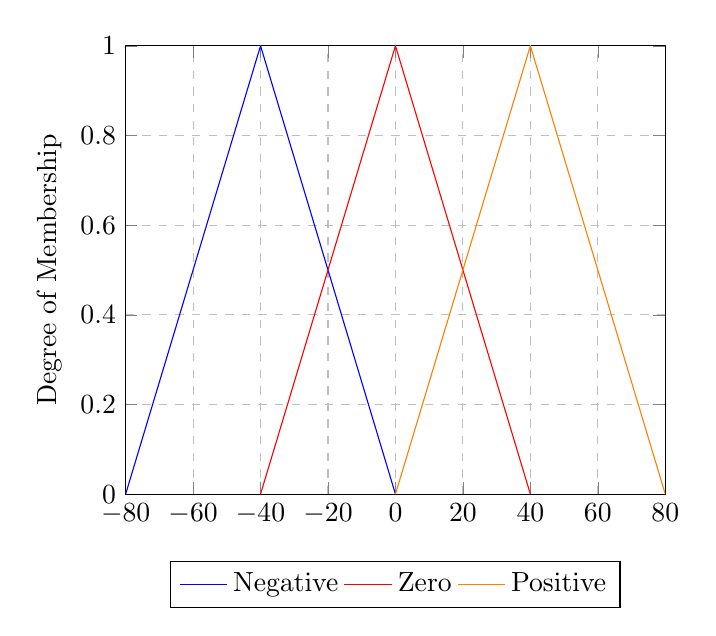
\begin{tikzpicture}
        \begin{axis}[
            ylabel={Degree of Membership},
            ymin=0, ymax=1,
            xmin=-80, xmax=80,
            legend style={at={(0.5,-0.15)},anchor=north,legend columns=-1},
            ymajorgrids=true,
            xmajorgrids=true,
            grid style=dashed
        ]
        
        % Negative Membership Function
        \addplot[solid, blue] coordinates {(-80,0) (-40,1) (0,0)};
        \addlegendentry{Negative}
        
        % Zero Membership Function
        \addplot[solid, red] coordinates {(-40,0) (0,1) (40,0)};
        \addlegendentry{Zero}
        
        % Positive Membership Function
        \addplot[solid, orange] coordinates {(0,0) (40,1) (80,0)};
        \addlegendentry{Positive}
        
        \end{axis}
    \end{tikzpicture}
    \caption{Membership Functions for Input Variable "Error"}
\end{figure}

We think, that this variable could model reality better, if we would use a trapezoidal membership function for the lowest and highest values, since for example if the error is bigger than 40 degrees, the error is positive, but the corresponding membership function start decreasing. This might influence the activation of some rules involving this variable, and the system might react as if the error is smaller than it actually is. Regardless, we followed the instructions and used a triangle membership function for the lowest and highest values.

\subsubsection{Error Derivative}

\begin{figure}[H]
    \centering
    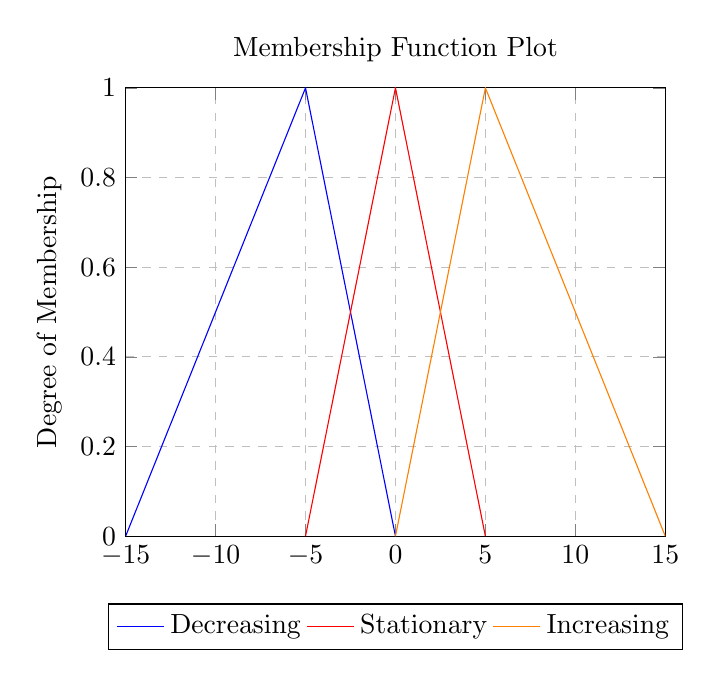
\begin{tikzpicture}
        \begin{axis}[
            title={Membership Function Plot},
            ylabel={Degree of Membership},
            ymin=0, ymax=1,
            xmin=-15, xmax=15,
            legend style={at={(0.5,-0.15)},anchor=north,legend columns=-1},
            ymajorgrids=true,
            xmajorgrids=true,
            grid style=dashed
        ]
        
        % Decreasing Membership Function
        \addplot[solid, blue] coordinates {(-15,0) (-5,1) (0,0)};
        \addlegendentry{Decreasing}
        
        % Stationary Membership Function
        \addplot[solid, red] coordinates {(-5,0) (0,1) (5,0)};
        \addlegendentry{Stationary}
        
        % Increasing Membership Function
        \addplot[solid, orange] coordinates {(0,0) (5,1) (15,0)};
        \addlegendentry{Increasing}
        
        \end{axis}
    \end{tikzpicture}
    \caption{Membership Functions for Input Variable "Error Derivative"}
\end{figure}

The previous observation is also valid for the Error Derivative variable. We used a triangle membership function for the lowest and highest values, but a trapezoidal membership function might be more accurate.
One additional comment is that when we used the original range of [-5, 5], the derivative frequently exceeded the bounds in the simulation, causing the fuzzy controller to output zero. We adjusted the range to [-15, 15] to obtain more accurate results.

\subsubsection{Thrust}

\begin{figure}[H]
    \centering
    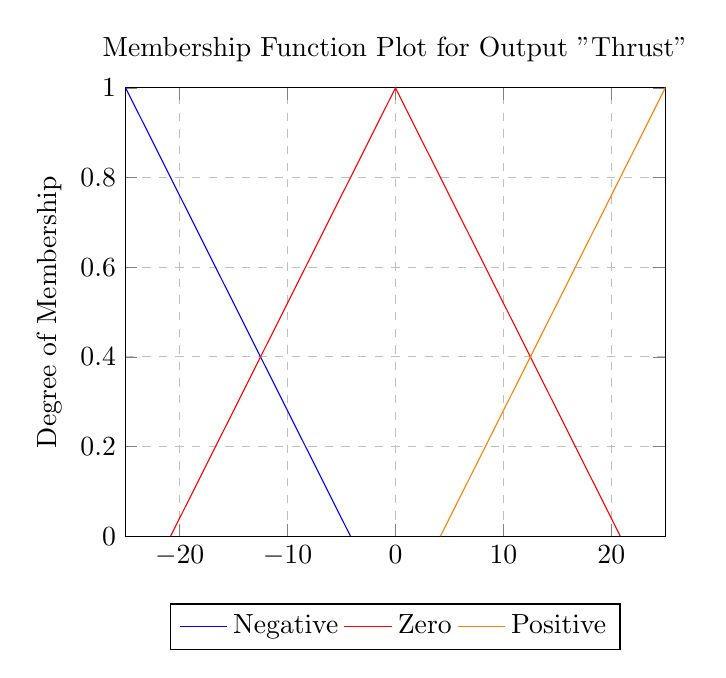
\begin{tikzpicture}
        \begin{axis}[
            title={Membership Function Plot for Output "Thrust"},
            ylabel={Degree of Membership},
            ymin=0, ymax=1,
            xmin=-25, xmax=25,
            legend style={at={(0.5,-0.15)},anchor=north,legend columns=-1},
            ymajorgrids=true,
            xmajorgrids=true,
            grid style=dashed
        ]
        
        % Negative Membership Function
        \addplot[solid, blue] coordinates {(-45.833,0) (-25,1) (-4.167,0)};
        \addlegendentry{Negative}
        
        % Zero Membership Function
        \addplot[solid, red] coordinates {(-20.833,0) (0,1) (20.833,0)};
        \addlegendentry{Zero}
        
        % Positive Membership Function
        \addplot[solid, orange] coordinates {(4.167,0) (25,1) (45.833,0)};
        \addlegendentry{Positive}
        
        \end{axis}
    \end{tikzpicture}
    \caption{Membership Functions for Output Variable "Thrust"}
\end{figure}

Since this membership function was not given, we designed it according to our previous observations, making the activation of the Negative and Positive variables the highest at the lowest and highest values, respectively. The three variables are evenly distributed in the given interval ([-25, 25]).

\subsection{Rules}

We designed the 9 rules required in the exercise as follows:

\begin{table}[h!]
    \centering
    \renewcommand{\arraystretch}{1.25} % Increase vertical space between rows
    \setlength{\tabcolsep}{10pt}      % Increase horizontal space between columns
    \begin{tabular}{|p{3cm}|p{4cm}|p{3cm}|}
    \hline
    \textbf{\large Error} & \textbf{\large ErrorDerivative} & \textbf{\large Thrust} \\ \hline
    \large Negative       & \large Decreasing                & \large Negative        \\ \hline
    \large Zero           & \large Decreasing                & \large Negative        \\ \hline
    \large Positive       & \large Decreasing                & \large Positive        \\ \hline
    \large Negative       & \large Stationary                & \large Negative        \\ \hline
    \large Zero           & \large Stationary                & \large Zero            \\ \hline
    \large Positive       & \large Stationary                & \large Positive        \\ \hline
    \large Negative       & \large Increasing                & \large Negative        \\ \hline
    \large Zero           & \large Increasing                & \large Positive        \\ \hline
    \large Positive       & \large Increasing                & \large Positive        \\ \hline
    \end{tabular}
    \caption{Rules and Corresponding Weights}
    \label{tab:rules}
\end{table}
    
When the Error is not \textit{Zero}, the Thrust is set accordingly: if the Error is \textit{Negative}, the Thrust is \textit{Negative}, if the Error is \textit{Positive}, the Thrust is \textit{Positive}. The Error Derivative variable is used to fine-tune the thrust, so if the Error is at the moment \textit{Zero}, but it is \textit{Increasing}, the thrust is \textit{Positive} and if the Error is \textit{decreasing}, the Thrust is \textit{Negative}. If the Error is \textit{Zero}, and it is \textit{Stationary} as well, we set the Thrust is \textit{Zero}.
    
\section{Results}

We ran the simulation for a stop time of 80 seconds with the provided controller and given parameters. The results are shown in the following figures:

\begin{figure}[h!]
    \centering
    \includegraphics[width=0.7\textwidth]{simulation1.jpg}
    \caption{theta\_ref = 20 and thrust = 0.123}
    \label{fig:simulation1}
\end{figure}
\vspace{1cm}

\begin{figure}[h!]
    \centering
    \includegraphics[width=0.7\textwidth]{simulation2.jpg}
    \caption{theta\_ref = -10 and thrust = -0.062}
    \label{fig:simulation2}
\end{figure}
\vspace{1cm}

In both cases, our designed control system was able to stabilize the pendulum at the desired angle. We don't see any oscillations, and the system reaches the desired angle in a reasonable time. We can clearly see how the thrust is adjusted according to the error and its derivative. 

\section{More complex controller}

To test out the cababilities of the fuzzy controller, we designed a more complex controller with 7 membership functions for the Thrust output variable. The plots frim the simulation are shown in figures \ref{fig:complex1} and \ref{fig:complex2}.

\begin{figure}[H]
    \centering
    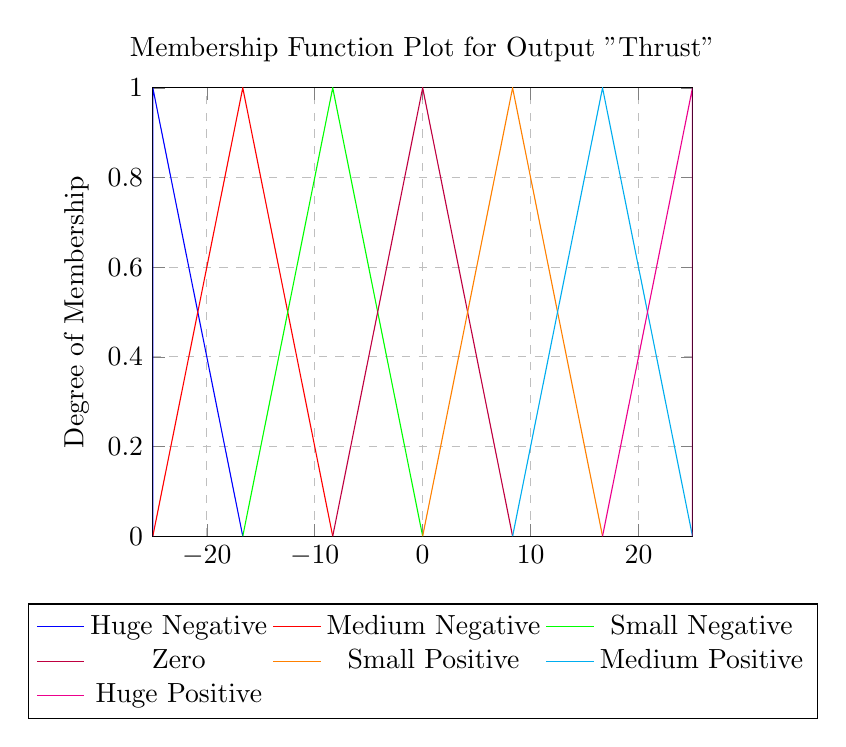
\begin{tikzpicture}
        \begin{axis}[
            title={Membership Function Plot for Output "Thrust"},
            ylabel={Degree of Membership},
            ymin=0, ymax=1,
            xmin=-25, xmax=25,
            legend style={at={(0.5,-0.15)},anchor=north,legend columns=3},
            ymajorgrids=true,
            xmajorgrids=true,
            grid style=dashed
        ]
        
        % Huge Negative Membership Function
        \addplot[solid, blue] coordinates {(-25,0) (-25,1) (-16.6667,0)};
        \addlegendentry{Huge Negative}
        
        % Medium Negative Membership Function
        \addplot[solid, red] coordinates {(-25,0) (-16.6667,1) (-8.3333,0)};
        \addlegendentry{Medium Negative}
        
        % Small Negative Membership Function
        \addplot[solid, green] coordinates {(-16.6667,0) (-8.3333,1) (0,0)};
        \addlegendentry{Small Negative}
        
        % Zero Membership Function
        \addplot[solid, purple] coordinates {(-8.3333,0) (0,1) (8.3333,0)};
        \addlegendentry{Zero}
        
        % Small Positive Membership Function
        \addplot[solid, orange] coordinates {(0,0) (8.3333,1) (16.6667,0)};
        \addlegendentry{Small Positive}
        
        % Medium Positive Membership Function
        \addplot[solid, cyan] coordinates {(8.3333,0) (16.6667,1) (25,0)};
        \addlegendentry{Medium Positive}
        
        % Huge Positive Membership Function
        \addplot[solid, magenta] coordinates {(16.6667,0) (25,1) (25,0)};
        \addlegendentry{Huge Positive}
        
        \end{axis}
    \end{tikzpicture}
    \caption{Membership Functions for Output Variable "Thrust"}
\end{figure}

To make a change, we need to modify the rules too. Here are the updated rules:

\begin{table}[h!]
    \centering
    \renewcommand{\arraystretch}{1.25} % Increase vertical space between rows
    \setlength{\tabcolsep}{10pt}      % Increase horizontal space between columns
    \begin{tabular}{|p{3cm}|p{4cm}|p{5cm}|}
    \hline
    \textbf{\large Error} & \textbf{\large ErrorDerivative} & \textbf{\large Thrust} \\ \hline
    \large Negative       & \large Decreasing               & \large Huge Negative    \\ \hline
    \large Zero           & \large Decreasing               & \large Small Negative   \\ \hline
    \large Positive       & \large Decreasing               & \large Medium Negative  \\ \hline
    \large Negative       & \large Stationary               & \large Medium Negative  \\ \hline
    \large Zero           & \large Stationary               & \large Zero             \\ \hline
    \large Positive       & \large Stationary               & \large Medium Positive  \\ \hline
    \large Negative       & \large Increasing               & \large Medium Negative  \\ \hline
    \large Zero           & \large Increasing               & \large Small Positive   \\ \hline
    \large Positive       & \large Increasing               & \large Huge Positive    \\ \hline
    \end{tabular}
    \caption{Fuzzy Logic Rules for Thrust Calculation}
    \label{tab:rules}
\end{table}

We've ran both simulations with this new controller, and the results are shown in the following figures:

\begin{figure}[h!]
    \centering
    \includegraphics[width=0.7\textwidth]{complex1.jpg}
    \caption{theta\_ref = 20 and thrust = 0.123}
    \label{fig:complex1}
\end{figure}
\vspace{1cm}

\begin{figure}[h!]
    \centering
    \includegraphics[width=0.7\textwidth]{complex2.jpg}
    \caption{theta\_ref = -10 and thrust = -0.062}
    \label{fig:complex2}
\end{figure}
\vspace{1cm}

Initially we thought that to see an improvement we would need to increase the the sensitivity of the input variables with more membership functions and more intricate rules, but we see a huge improvement with changing just the output variable. It reaches the desired angle much faster, while perfectly maintaining stability. Further work could be done to optimize the input variables as well, but the results are already very promising.

\section{Conclusions}  

In this study, we successfully designed and implemented a Mamdani fuzzy inference system (FIS) to control a compound pendulum, achieving significant improvements in stability and transient response compared to the open-loop system. The fuzzy controller effectively reduced oscillations and achieved the desired angular position, demonstrating robustness and adaptability. By experimenting with enhanced membership functions and a more granular rule base, we observed that increasing the complexity of the output variable improved response speed and stability without requiring additional adjustments to input variables. This highlights the potential of fuzzy logic systems to handle nonlinear control problems efficiently. The results underscore the versatility and practicality of fuzzy computing in real-world dynamic systems.

\section{Usage of generative AI models}

We used ChatGPT for spelling checks, grammar corrections, and sentence structure improvements. 

\end{document}